\documentclass[letterpaper, reqno,11pt]{article}
\usepackage[margin=1.0in]{geometry}
\usepackage{color,latexsym,amsmath,amssymb,graphicx, float}
\usepackage{hyperref}

\hypersetup{
colorlinks=true,
linkcolor=magenta,
filecolor=magenta,
urlcolor=cyan,
}

\graphicspath{ {images/} }

\begin{document}
\pagenumbering{arabic}
\title{Phys 350 Homework 1}
\date{22/01/22}
\author{Xander Naumenko}
\maketitle

{\noindent\bf Question 1.} Expanding the left side of the equation: 

\[
\vec a\times(\vec b\times\vec c)=\vec e_x\times\left( (b_yc_z-b_zc_y)\vec e_x+(b_zc_x-b_xc_z)\vec e_y+(b_xc_y-b_yc_x)e_z \right)= (b_zc_x-b_xc_z)\vec e_z+(b_yc_x-b_xc_y)\vec e_y
.\] 
Similarly expanding the right side of the equation: 

\[
\vec b(\vec a\cdot\vec c)-\vec c(\vec a\cdot\vec b)=\vec b(c_x)-\vec c(b_x)=(b_yc_x-b_xc_y)\vec e_y+(b_zc_x-b_xc_z)\vec e_z
.\] 
Since the left and right hand sides of the equation are the same one expanded, the equality is true for the original form as well. 

To argue that this holds in general, note that everything is symmetric regardless of whether $\vec a=\vec e_x$, $\vec a=\vec e_y$ or $\vec a=\vec e_z$, so what we just showed holds true for any of the aformentioned choices of $\vec a$. Using this, we find that 

\[
\vec a\times(\vec b\times\vec c)=a_x\vec e_x\times(\vec b\times\vec c)+a_y\vec e_y\times(\vec b\times\vec c)+a_z\vec e_z\times(\vec b\times\vec c)
.\] 

\[
=\vec b(a_x\vec e_x\cdot\vec c)-\vec c(a_x\vec e_x\cdot\vec b)+\vec b(a_y\vec e_y\cdot\vec c)-\vec c(a_y\vec e_y\cdot\vec b)+\vec b(a_z\vec e_z\cdot\vec c)-\vec c(a_z\vec e_z\cdot\vec b)
.\] 

\[
=\vec b(\vec a\cdot\vec c)-\vec c(\vec a\cdot\vec b)
\] 
as required. 

{\noindent\bf Question 2.} In cartesian coordinates, the speed is 

\[
\vec v(t)=\begin{pmatrix} \frac{3}{5}\cos(t^2)-\frac{6}{5}t^2\sin(t^2)\\ \frac{3}{5}\sin(t^2)+\frac{6}{5}t^2\cos(t^2)\\ \frac{4}{5} \end{pmatrix}  
.\] 
To find the velocity in cylindrical coordinates, first convert to cylindrical: 

\[
    r=\sqrt{x^2+y^2} =\frac{3}{5}t
\]
\[
\phi=\tan \frac{y}{x}=\tan\left( \arctan(t^2) \right) =t^2
\]

\[
z=z=\frac{4}{5}t
.\]
Thus the velocity in cylindrical is 

\[
\dot r=\frac{3}{5}
\]
\[
\dot \phi = 2t
\]
\[
\dot z=\frac{4}{5}
.\]
For acceleration, differentiate the cartesian velocity: 

\[
\vec a(t)=\begin{pmatrix} -\frac{6}{5}t\sin(t^2)-\frac{12}{5}t \sin(t^2)-\frac{12}{5}t^3 \cos(t^2) \\ \frac{6}{5}t\cos(t^2)+\frac{12}{5}t \cos(t^2)-\frac{12}{5}t^3 \sin(t^2) \\ 0 \end{pmatrix}
.\]
For cylindrical, the differentiation is much simpler: 

\[
\ddot r=0
.\]
\[
\ddot\phi = 2
.\]
\[
\ddot z = 0
.\]
Using Newton's second law $\vec F=m\vec a$ where $\vec a$ is the acceleration in either cylindrical or cartesian coordinates that we just found above. 

{\noindent\bf Question 3i.} Taking each of the derivatives separately: 

\[
    \frac{\partial f}{\partial q} =e^{\dot q t}, \frac{\partial f}{\partial \dot q}=qte^{\dot qt},\frac{\partial f}{\partial t} =q\dot qe^{\dot qt}, \frac{df}{dt}\left( \frac{\partial f}{\partial \dot q}  \right) =qe^{\dot qt}+q\dot qte^{\dot qt}
.\]
The total derivative is 

\[
\frac{df}{dt}=\frac{\partial f}{\partial t} +\frac{\partial f}{\partial q} \dot q+\frac{\partial f}{\partial \dot q} \ddot q=q\dot qe^{\dot qt}+\dot qe^{\dot q t}+qt\ddot qe^{\dot qt}
.\]
Next to plug in $q(t)=\frac{t}{t+1}$, we find the derivatives of $ q$: 

\[
\dot q=\frac{1}{(t+1)^2}, \ddot q=\frac{-2}{(t+1)^3}
.\]
Plugging this into the expression for the total derivative: 

\[
\frac{df}{dt}=\left(\frac{t}{(t+1)^3}+\frac{1}{(t+1)^2}-\frac{2t^2}{(t+1)^4}\right)e^{\frac{t}{(t+1)^2}}=\left( \frac{2t+1}{(t+1)^4} \right) e^{\frac{t}{(t+1)^2}}
.\]
Verifying by plugging $q$ into the original expression, we get 

\[
\frac{df}{dt}=\frac{d}{dt}\left( \frac{t}{t+1}e^{\frac{t}{(t+1)^2}} \right)=\left(\frac{t}{(t+1)^3}+\frac{1}{(t+1)^2}-\frac{2t^2}{(t+1)^4}\right)e^{\frac{t}{(t+1)^2}}=\left( \frac{2t+1}{(t+1)^4} \right) e^{\frac{t}{(t+1)^2}}
.\]

{\noindent\bf Question 3ii.} Following the exact same steps as the previous part, we find the partial derivatives: 

\[
\frac{\partial f}{\partial q} =2tq+\cos(\dot q^2), \frac{\partial f}{\partial \dot q} =-2q\dot q \sin(\dot q^2), \frac{d}{dt}\left( \frac{\partial f}{\partial \dot q} \right) =-2\dot q^2 \sin(\dot q^2)-2q\ddot q\sin(\dot q^2)+4q\dot q\ddot q\cos(\dot q^2)
.\]
The total derivative is 
\[
\frac{df}{dt}=\frac{\partial f}{\partial t} +\frac{\partial f}{\partial q} \dot q+\frac{\partial f}{\partial \dot q} \ddot q=q^2+2tq\dot q+\dot q\cos(\dot q^2)-2q\dot q\ddot q \sin(\dot q^2)
.\]
For the specific case of the given $q$, we find that 
\[
\frac{df}{dt}=\frac{t^2}{(t+1)^2}+\frac{2t^2}{(t+1)^3}+\frac{1}{(t+1)^2}\cos\left(\frac{1}{(t+1)^4}\right)+\frac{4t}{(t+1)^6}\sin\left( \frac{1}{(t+1)^4} \right) 
.\]
To verify this we plug $q$ in to the original expression and find the derivative that way: 
\[
\frac{df}{dt}=\frac{d}{dt}\left( \frac{t^3}{(t+1)^2}+\frac{t}{t+1}\cos\left(\frac{1}{(t+1)^4}\right) \right) 
.\]
\[
=\frac{t^2}{(t+1)^2}+\frac{2t^2}{(t+1)^3}+\frac{1}{(t+1)^2}\cos\left(\frac{1}{(t+1)^4}\right)+\frac{4t}{(t+1)^6}\sin\left( \frac{1}{(t+1)^4} \right) 
.\]

{\noindent\bf Question 4i.} From the definition of the cross product, we know that $|\vec a\times\vec b|=|\vec a| |\vec b|\sin\theta$, where $\theta$ is the angle between the vectors. From figure 1a. in the problem statement it is clear that the surface generated by the two vectors is a parrallelogram, whose area is it's base length times its height. Taking $\vec a$ to be it's base, it has base length $|\vec a|$ and height $\sin\theta|\vec b|$, so its area is 

 \[
A=|\vec a| |\vec b|\sin\theta=|\vec a\times\vec b
\]
as required. 

{\noindent\bf Question 4ii.} By the definition of dot product we have that $\vec a\cdot\vec d=|\vec a| |\vec d|\cos\theta$, where again $\theta$ is the angle between the two vectors. From the previous part we know that $|\vec b\times\vec c|$ represents the area of the parrallelogram generated by $\vec b$ and $\vec c$, i.e. the base of the parrallelopiped in figure 1b. in the problem statement. The direction of the cross product is perpendicular to both $\vec b$ and $\vec c$, so the height of the volume is $|\vec a|\cos\theta$, where $\theta$ is the angle between $\vec a$ and $|\vec b\times\vec c|$. Thus the volume of the parrallelopiped is 

\[
V=|\vec b\times\vec c| |\vec a|\cos\theta=\vec a\cdot (\vec b\times \vec c)
.\]

Since the argument holds the same completely symmetrically among $\vec a, \vec b$ and $\vec c$ as long as the pair of vectors inside the product yield a positive result, it is also true that $V=\vec b\cdot (\vec c\times\vec a)=\vec c\cdot(\vec a\times\vec b)$. 

{\noindent\bf Question 5.} A free body diagram of the situation can be seen in figure \ref{fig:q5}. First we balance the forces of the smaller block: 

\[
\sum F_y=0\implies F_{gm}-F_{N}\cos\theta=m a\sin\theta
.\]
\[
\sum F_x=0\implies F_{N}\sin\theta=m(a\cos\theta-a_x)
.\]

\begin{figure}[htpb]
    \centering
    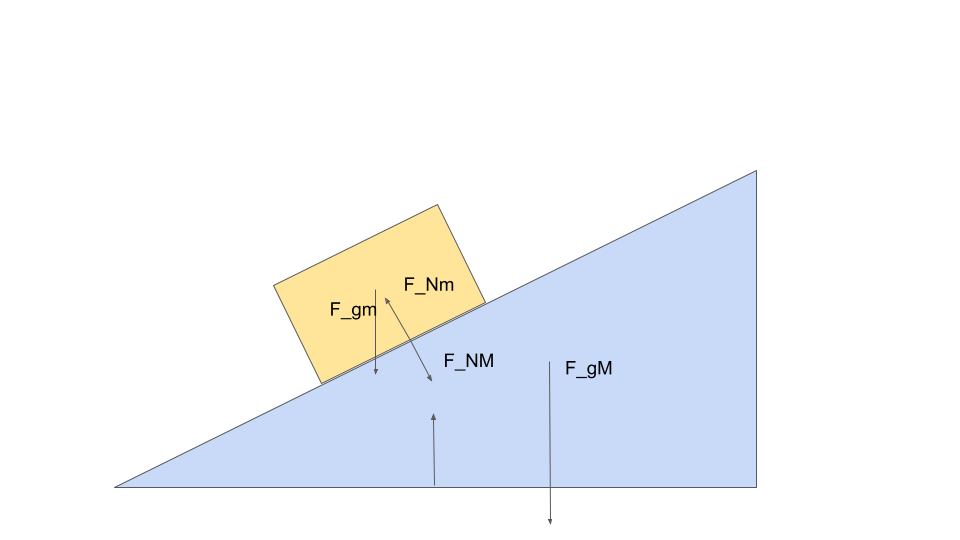
\includegraphics[width=0.8\textwidth]{q5}
    \caption{Free body diagram for question 5}
    \label{fig:q5}
\end{figure}

For the larger block, we get a different set of equations: 

\[
\sum F_x=0\implies F_N\sin\theta=Ma_x
.\]
Note that equilibrium in the $y$ direction isn't relevant since there is not friction. 

Putting these equations together and solving: 

\[
    (M+m)a_x=ma\cos\theta\implies a=(\frac{M}{m}+1)a_x \sec\theta
.\]
\[
    mg-Ma_x\cot\theta=(M+m)a_x\tan\theta\implies a_x=\frac{mg}{M\cot\theta+(M+m)\tan\theta}
.\]
\[
a=\frac{(M+m)mg}{M\cos\theta\cot\theta+(M+m)m\sin\theta}
.\]




\end{document}
